% !TeX root = ../libro.tex
% !TeX encoding = utf8

\chapter{Aprendizaje de características}

La efectividad de los métodos de aprendizaje automático depende en gran medida de la representación de los datos utilizada. La obtención de una buena representación es crucial en el proceso de aprendizaje. Dicha tarea es una de las que más tiempo consumen en cualquier proyecto de esta área~\cite{domingos2012few}. El desarrollo de técnicas que permitan la obtención de buenas representaciones automáticamente se ha convertido en un importante campo dentro del aprendizaje automático. A este conjunto de técnicas se le denomina aprendizaje de características o de representación.~\cite{bengio2013representation}.

Obtener representaciones mejores para la aplicación de técnicas de aprendizaje no es el único motivo para la aplicación del aprendizaje de características. En muchas aplicaciones la obtención de características es la meta en sí. Algunos ejemplos de esto son la representación de documentos en códigos binarios compactos que faciliten su búsqueda~\cite{salakhutdinov2009semantic}, compresión de imágenes minimizando la pérdida de información~\cite{theis2017lossy}, la transformación del dominio de un problema a otro diferente~\cite{deng2013sparse} o la generación de imágenes restauradas a partir de versiones distorsionadas~\cite{xie2012image}.

En el caso de este trabajo se aplica esta idea a la manipulación y generación de melodías musicales. Estas son datos de naturaleza compleja, difíciles de manejar de forma rápida y efectiva, y más aún con la inmediatez que requiere una interpretación en directo. Utilizaremos melodías monofónicas de dos compases de 4/4, es decir, como máximo una nota suena a la vez y hay cuatro pulsos por compás. Supongamos además, con afán de simplificación, que la máxima subdivisión posible para dichas melodías es la semicorchea (un cuarto de pulso) e ignoremos el tempo al que se interpreta la secuencia y el volumen. Si suponemos que las notas diferentes posibles son las 88 que tienen los pianos actuales y que en cada pulso podemos tocar una de las 88 teclas, levantar la tecla que se venía tocando o realizar un silencio, esto nos deja 90 posibles acciones para cada semicorchea. Necesitaríamos entonces 7 bits por semicorchea para su cifrado, y tenemos 32 semicorcheas por melodía. Explorar todas las posibilidades bit a bit es una tarea intratable y la mayoría de melodías obtenidas serían incoherentes ~\cite{roberts2018learning}.

El objetivo será por tanto obtener una representación de estas melodías fácil de manipular por parte del artista, que permita un acercamiento diferente a la composición y la interpretación. Para ello será clave la extracción de representaciones de baja dimensionalidad.

\section{Selección de características}
El precedente para la extracción de características se encuentra en la selección de características para problemas de aprendizaje automático. En los últimos años del número de características utilizadas ha crecido desde las pocas decenas hasta las miles o decenas de miles~\cite{guyon2003introduction}. Con este crecimiento surge también la necesidad de seleccionar aquellas características más útiles para la tarea que se pretende afrontar.

La selección de características consiste en seleccionar un subconjunto de entre las características disponibles para mejorar la tarea de aprendizaje. Existen muchos beneficios potenciales que pueden derivarse de esta acción: facilitar la visualización y entendimiento de los datos, disminución de los recursos computacionales necesarios, tanto en espacio de memoria para almacenaje de datos como en tiempo de cómputo en el entrenamiento y predicción, o evitar la maldición de la dimensionalidad (\textit{the curse of dimensionality}) que obstaculiza o imposibilita el aprendizaje cuando se cuenta con pocos ejemplos y un número de características elevado~\cite{beyer1999nearest}.

Un primer acercamiento a la selección de características consiste en la jerarquización de variables utilizando alguna métrica del valor de cada variable para el aprendizaje y descartando las menos útiles. Es una técnica ampliamente usada por su simplicidad, escalabilidad y buen desempeño empírico, pero presenta un problema importante. La mayoría de las veces la utilidad de una variable no puede juzgarse individualmente, y la inclusión de variables que resultan redundantes por sí solas pueden producir una mejora significativa de los resultados por su relación con otras.

Como respuesta a este hecho surgen métodos que no tratan de seleccionar características individualmente, sino conjuntos de características. De entre estos podemos distinguir tres categorías:

\begin{itemize}

  \item Métodos de filtro: seleccionan el subconjunto de características como paso de preprocesamiento de datos, independientemente del predictor elegido.
  \item Métodos de envoltura: utilizan el desempeño de un algoritmo de aprendizaje automático para medir la utilidad del subconjunto seleccionado. Su alto coste computacional implica que una búsqueda exhaustiva sea imposible en la práctica, por lo que la estrategia de búsqueda utilizado es clave en este tipo de métodos.
  \item Métodos integrados: realizan la selección de características durante el aprendizaje y son específicos del algoritmo de aprendizaje usado.

\end{itemize}

\section{Extracción de características}

Frente a la selección de entre las características ya existentes aparece una perspectiva diferente: la creación de nuevas representaciones a partir de la existente, no solo mediante la selección sino mediante la generación de nuevas características a través de transformaciones de las iniciales. Surge no solo con la intención de generar representaciones más eficientes para el aprendizaje, sino también más comprensibles y fáciles de manejar.

Puede pasar que todas las características de los datos sean relevantes, y aún así la dimensionalidad de los mismos sea todavía demasiado elevada. Descubrir las dependencias entre las características puede permitir reducir dicha dimensionalidad. Cuando dos características están altamente correladas, conocer información sobre una implica conocer información sobre la otra. En lugar de eliminar arbitrariamente una de estas características, una manera de reducir la dimensionalidad es obtener una  representación a partir de una transformación de dichas características. Esta perspectiva viene motivada por el hecho de que las dependencias entre variables pueden ser muy complejas, y eliminar una de ellas puede resultar en perder parte de la información que ambas comunican~\cite{lee2007nonlinear}.

El nuevo conjunto de características por lo general debe tener un número menor de variables pero debe preservar la información del conjunto inicial. Se buscan por tanto transformaciones de las variables con unas propiedades tales que se asegure que la transformación no altera la información que contenían las variables iniciales, solo su representación.

Estas transformaciones pueden intentar cumplir dos objetivos diferentes. El primero, y más simple, es detectar y eliminar dependencias. Para ello la transformación debe reducir el número de variables. El segundo, y más complejo, es recuperar las variables latentes, esto es, aquellas que son el origen de las observadas, pero que no pueden medirse directamente.

La construcción de una representación nueva podría considerarse una tarea muy específica del dominio de la información que se trata, y puede ser la manera de introducir conocimiento específico sobre dicho dominio. Sin embargo, se han desarrollado gran cantidad de técnicas genéricas para la construcción de nuevas representaciones.
En esta sección se repasan algunas de ellas. Se explicarán algunas de las técnicas tradicionales para después hacer especial hincapié en aquellas para las que se aplica aprendizaje profundo.

\subsection{Técnicas tradicionales de extracción de características}

Podemos separar las técnicas entre aquellas que realizan transformaciones lineales de los datos de entrada y las que realizan transformaciones no lineales. De entre las técnicas lineales la más extendida es el análisis de componentes principales.

% Mencionar: (Lineales: PCA, LDA. No lineales: Isomap, LLE)

El análisis de componentes principales (\textit{principal component analysis}, PCA) se base en la asunción de que las $D$ variables observadas, expresadas en el vector aleatorio $\textbf{Y} = (Y_1,...,Y_D)^T$ son el resultado de una transformación lineal $\textbf{W}$ de variables $P$ latentes desconocidas, $\textbf{X} = (X_1,...,X_M)^T$: $$\textbf{Y} = \textbf{W}\textbf{X}.$$ Se asume también que todas las variables latentes tienen una distribución normal, y que la transformación $\textbf{W}$ es un cambio de ejes, es decir, que sus columnas son ortogonales entre sí y tienen norma unitaria. En definitiva, $\textbf{W} \in \mathcal{M}_{D \times P}$, con $\textbf{W}^T\textbf{W} = \textbf{I}_P$. Por último, pero menos restrictivo, PCA asume que las variables observadas ${y}$ y las variables latentes $\textbf{x}$ están centradas, es decir, $E[\textbf{X}] = 0_D$ y $E[\textbf{Y}] = 0_P$.

A partir de estas condiciones se pretende obtener la dimensión $P$ y la transformación $\textbf{W}$ a partir de un conjunto de $N$ observaciones del vector aleatorio $\textbf{Y}$, que pueden expresarse como una matriz $$Y = [\textbf{Y}^{(1)},...,\textbf{Y}^{(N)}].$$

Si asumimos que las variables de $\textbf{X}$ son incorreladas, es decir, que la matriz de covarianzas $Cov(\textbf{X}) = E[\textbf{X}\textbf{X}^T]$ es diagonal. Tras la transformación por $\textbf{W}$ las variables de $\textbf{y}$ sí estarán correladas, y su matriz de covarianzas no será diagonal. El objetivo de PCA es obtener las $P$ variables incorreladas de $\textbf{X}$ a través de las de $\textbf{Y}$. Podemos expresar la matriz de covarianzas de $\textbf{Y}$ como $$Cov(\textbf{Y}) = E[\textbf{Y}\textbf{Y}^T] = E[\textbf{W}\textbf{X}\textbf{X}^T\textbf{W}^T] = \textbf{W}E[\textbf{X}\textbf{X}^T]\textbf{W}^T = \textbf{W}Cov(\textbf{X})\textbf{W}^T.$$ Como $\textbf{W}^T\textbf{W} = \textbf{I}$, multiplicando a la izquierda por $\textbf{W}^T$ y a la derecha por $\textbf{W}$ obtenemos $$Cov(\textbf{X}) = \textbf{W}^TCov(\textbf{Y})\textbf{W}. $$ Podemos entonces factorizar la matriz Cov(\textbf{Y}), que por ser simétrica es diagonalizable, como $$ Cov(\textbf{Y}) = \textbf{V}\textbf{A}\textbf{V}^T,$$ donde \textbf{V} es una matriz de vectores propios normalizados $\textbf{v}_d$ y $\textbf{A}$ es una matriz diagonal con los valores propios asociados $\lambda_d$, en orden descendiente. Como la matriz de covarianzas es simétrica y semidefinida positiva los vectores propios son ortogonales y los valores propios son reales no negativos. Sustituyendo en la expresión de $Cov(\textbf{X})$ obtenemos $$Cov(\textbf{X}) = \textbf{W}^T\textbf{V}\textbf{A}\textbf{V}^T\textbf{W},$$ donde, en el caso ideal en el que todas las hipótesis son respetadas y las observaciones no tienen ruido, solo los primeros $P$ valores propios en $\textbf{A}$ son positivos, siendo el resto nulos. Tomamos entonces los vectores propios asociados a estos $P$ valores, $$\textbf{W} = \textbf{V}\textbf{I}_{D \times P},$$ obteniendo así $$Cov(\textbf{X}) = \textbf{I}_{P \times D}\textbf{A}\textbf{I}_{D \times P}.$$ Esto significa que los valores propios en $\textbf{A}$ se corresponden con las varianzas de las variables latentes.

En la práctica los datos observados serán ruidosos y por tanto todos los valores propios de $Cov(\textbf{Y})$ serán mayores que cero, por lo que la elección de las $P$ columnas en $\textbf{V}$ es más complicada. Si las variables latentes tienen varianzas mayores que el ruido, basta tomar los vectores correspondientes a los mayores valores propios.

Desde un punto de vista geométrico, las columnas de $\textbf{V}$ indican las direcciones en $\mathbb{R}^D$ sobre las que se extiende el subespacio de las variables latentes. Si llamamos a estas columnas componentes, la elección de las columnas asociadas a las mayores varianzas es la elección de las componentes principales.

En una situación real la covarianza de $\textbf{Y}$ no es conocida, pero puede ser aproximada mediante la covarianza de la muestra: $$Cov(Y) = \frac{1}{N}YY^T.$$

Otra técnica lineal muy extendida es el análisis discriminante lineal. En este caso se trata de un método supervisado para datos clasificados. Genera una representación de los datos con una dimensión menor que respeta la estructura de clases y maximiza la separación entre las mismas. Es habitual aplicarla tras PCA~\cite{ye2005two}.

En cuanto a las técnicas que utilizan transformaciones no lineales, el escalamiento multidimensional (\textit{multidimensional scaling}, MDS) es una técnica que además sirve como base para otros algoritmos. Consiste en encontrar nuevas coordenadas en un espacio de menor dimensión manteniendo las distancias relativas entre los datos de manera lo más fiel posible. Isomap se basa en MDS, extendiéndolo para encontrar coordenadas que describan los verdaderos grados de libertad de los datos mientras que se preservan las distancias entre puntos. Por último la máquina de Boltzmann restringida (\textit{restricted boltzmann machine}, RMB) es un modelo que cuenta con una capa oculta y una visible. Están definidas por una distribución de probabilidad conjunta determinada por una función de energía. Son una alternativa para la inicialización de \textit{autoencoder} por capas, que veremos a continuación.

\subsection{Autoencoder}

Los \textit{autoencoder} (AE) son redes neuronales con una estructura simétrica, entrenados para reconstruir la entrada en la salida. La capa central representa la codificación de los datos de entrada. Por tanto, en este caso el interés no se encuentra en la salida de la red sino en la codificación obtenida mediante la misma. El objetivo del \textit{autoencoder} es obtener una representación de los datos de entrada con determinadas características, que estarán determinadas por la arquitectura de la red. Podemos por tanto considerar la estructura básica reflejada en \autoref{fig:basic-ae}: la entrada $\textbf{x}$ que se aplica en la codificación $\textbf{h}$ mediante el codificador (\textit{encoder}), representado por $f$, y la reconstrucción $\textbf{r}$, obtenida a partir de $\textbf{y}$ mediante el decodificador (\textit{decoder}), representado por $g$~\cite{goodfellow2016}.

\begin{figure}[htpb]
  \centering
  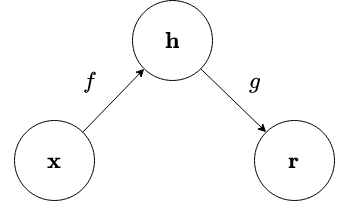
\includegraphics[width=0.6\textwidth]{basic-ae}
  \caption{Estructura básica de un \textit{autoencoder}}
  \label{fig:basic-ae}
\end{figure}

El \textit{autoencoder} más básico es una red prealimentada profunda con esta estructura. Puesto que se copia la entrada $\textbf{x}$ en la salida $\textbf{r}$, ambas tendrán la misma dimensión. La codificación $\textbf{y}$ es variable, y puede tener una dimensión menor o mayor en función de las propiedades deseadas en la representación de los datos de entrada. Tanto el codificador como el decodificador pueden tener tantas capas como sean necesarias, normalmente dispuestas de manera simétrica. Un ejemplo de red prealimentada profunda de esta forma puede observarse en la \autoref{fig:autoencoder}.

\begin{figure}[htpb]
  \centering
  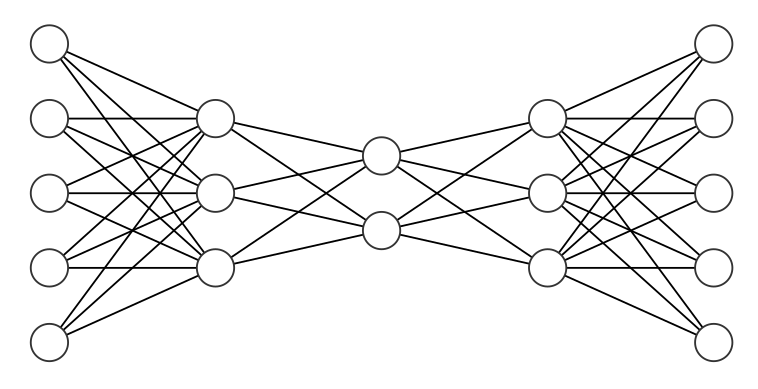
\includegraphics[width=0.8\textwidth]{autoencoder}
  \caption{Estructura de un \textit{autoencoder} como red prealimentada profunda}
  \label{fig:autoencoder}
\end{figure}

\subsubsection{Arquitecturas}

Los diferentes tipos de \textit{autoencoders} pueden ser clasificados según múltiples criterios. En este apartado se repasan las diferentes estructuras que puede tomar la red. Todas ellas son simétricas, con el codificador y el decodificador teniendo el mismo número de capas y de unidades en cada capa, en orden inverso. Puede considerarse que el codificador empieza en la entrada y tiene su salida en la codificación, que es la entrada del decodificador. La salida de este es la reconstrucción. Por tanto ambas estructuras comparten la capa de codificación. En función de las dimensiones de esta capa podemos considerar dos tipos de red:

\begin{itemize}
\item Incompleto (\textit{undercomplete}): la capa de codificación tiene dimensión menor que la de la entrada (y por tanto también que la salida). El menor número de unidades supone una restricción en la red, por lo que durante el entrenamiento el \textit{autoencoder} aprenderá una representación más compacta de la entrada. Cuando se tiene esta estructura la capa de codificación suele llamarse cuello de botella.
\item Sobrecompleto (\textit{overcomplete}): la capa de codificación tiene una dimensión igual o mayor a la de la entrada. Puede permitir que el \textit{autoencoder} aprenda la función identidad para copiar la entrada en la salida, por lo que suelen aplicarse otras restricciones. Mediante estas puede obtenerse también una representación compacta de los datos.
\end{itemize}

Además del número de unidades por capa, también pueden clasificarse los \textit{autoencoders} según la cantidad de capas que tienen. Así, podemos distinguir dos cateogrías:

\begin{itemize}
\item Superficial (\textit{shallow}): cuenta solamente con las capas de entrada, codificación y salida. Es la estructura más simple posible, pues tiene una única capa oculta, la capa de codificación.
\item Profundo (\textit{deep}): tiene más de una capa oculta. Puede ser entrenado capa a capa como si se tratara de varios \textit{autoencoders} superficiales superpuestos o como una única red profunda, como se explica en la \autoref{entrenamiento-ae}.
\end{itemize}

\begin{figure}
    \centering
    \begin{minipage}{0.45\textwidth}
        \centering
        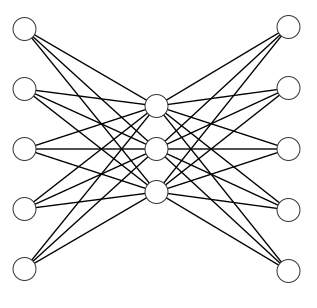
\includegraphics[width=1.1\textwidth]{undercomplete-shallow}
        \caption{\textit{Autoencoder} incompleto superficial}
    \end{minipage}\hfill
    \begin{minipage}{0.45\textwidth}
        \centering
        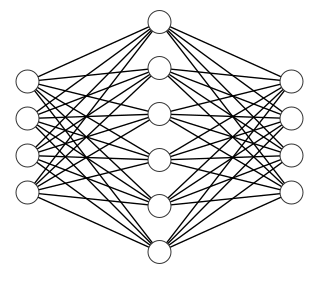
\includegraphics[width=1.1\textwidth]{overcomplete-shallow}
        \caption{\textit{Autoencoder} sobrecompleto superficial}
    \end{minipage}
\end{figure}

\begin{figure}
    \centering
    \begin{minipage}{0.45\textwidth}
        \centering
        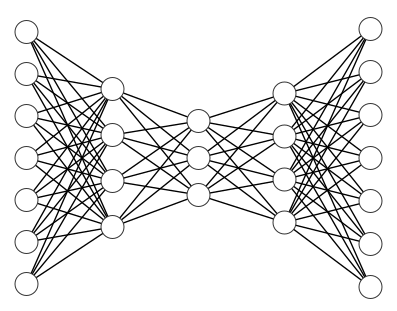
\includegraphics[width=1.2\textwidth]{undercomplete-deep}
        \caption{\textit{Autoencoder} incompleto profundo}
    \end{minipage}\hfill
    \begin{minipage}{0.45\textwidth}
        \centering
        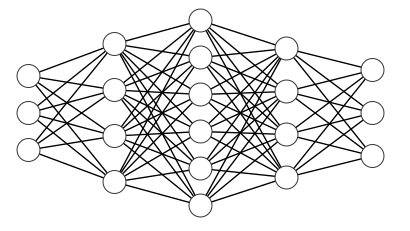
\includegraphics[width=1.2\textwidth]{overcomplete-deep}
        \caption{\textit{Autoencoder} sobrecompleto profundo}
    \end{minipage}
\end{figure}

\subsubsection{Funciones de activación más comunes}

Las unidades de activación generalmente utilizadas en los \textit{autoencoder} son las ya vistas en \autoref{unidades-ocultas}. Cuando se utilizan unidades de activación lineal con una sola capa oculta de $k$ unidades y se minimiza el error cuadrático medio, el modelo es equivalente a obtener las $k$ componentes principales mediante PCA.

Las unidades ReLU, muy utilizadas en muchos modelos de aprendizaje profundo, pueden resultar menos útiles para los \textit{autoencoder}. Puesto que su salida es nula para todos los valores negativos dificultan el proceso de reconstruir la entrada en la salida. Existe una alternativa reciente, las unidades lineales exponenciales escaladas (\textit{Scaled Exponential Linear Units}, SELU)~\cite{klambauer2017self}, cuya función de activación es

$$g(\textbf{z})_i = \lambda \left\{ \begin{array}{lcc}
             \alpha (e^x - 1) &   si  & x \leq 0
             \\ x &  si & x > 0
             \end{array}
   \right.,$$
con $\lambda > 1$.

\begin{figure}[htpb]
  \centering
  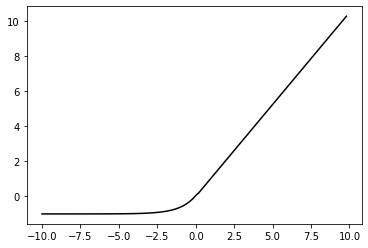
\includegraphics[width=0.6\textwidth]{selu}
  \caption{Gráfica de la función de activación de una SELU}
  \label{fig:selu}
\end{figure}

Es por esto que, en general, las funciones de activación más usadas son las sigmoides, tanto la función logística como la tangente hiperbólica.

\subsubsection{Función de coste}

La función de coste $J(W,b;S)$ del \textit{autoencoder} se calcula como la suma de las funciones de coste para cada elemento del conjunto de entrenamiento $L: \mathbb{R}^d \times \mathbb{R}^d \rightarrow \mathbb{R}$. Así, $$J(W,b;S) = \sum_{x \in S}L(x,(g \circ f)(x)),$$ donde $S$ es el conjunto de entrenamiento y $f$ y $g$ las funciones del codificador y decodificador respectivamente, determinadas por los pesos $W$ y los sesgos $b$. El objetivo será por tanto aprender $W$ y $b$ para minimizar $J$. La función $L$ suele tomarse como la log-verosimilitud negativa del ejemplo $x$ dada la salida $(g \circ f)(x)$.

\subsubsection{Entrenamiento}\label{entrenamiento-ae}

Para la optimización de \textit{autoencoders} pueden aplicarse los algoritmos vistos en la \autoref{optimizacion} basados en el descenso del gradiente como el descenso del gradiente estocástico y variantes como AdaGrad, RMSProp y Adam. Para el cálculo del gradiente se usa el algoritmo de propagación hacia atrás, también visto en la \autoref{back-propagation}.

Al igual que en los modelos de aprendizaje profundo del anterior capítulo, puede añadirse un término de regularización en la función de coste para evitar sobreajuste. Este término puede introducirse de distintas maneras, pero en general depende de los pesos para reducir su tamaño.

Conforme aumenta la profundidad de los \textit{autoencoders} el proceso de entrenamiento depende cada vez más de la inicialización de los pesos, ya que su número aumenta. Esta inicialización puede realizarse superponiendo sucesivos \textit{autoencoders} superficiales y entrenándolos capa a capa. Así, se comienza entrenando la primera capa oculta como si se tratara de un único \textit{autoencoder} superficial. La segunda capa se entrena de igual manera, tomando la salida de la primera capa como entrada, y así hasta haber completado todas las capas hasta llegar a la de codificación. Con esto se consigue una inicialización de los pesos para todas las capas del codificador. Las capas del decodificador se inicializan con la trasposición de los pesos de su capa simétrica. Finalmente puede realizarse un entrenamiento normal.

\subsection{Autoencoder variacional}

Los modelos descritos hasta el momento tienen su principal utilidad en generar representaciones más compactas de los datos de entrada. En contraposición, el \textit{autoencoder} variacional (\textit{variational autoencoder}, VAE) es un modelo generativo (\cite{kingma2013auto}, \cite{rezende2014stochastic}). Los modelos generativos aprenden una distribución de probabilidad de la que generar nuevos datos diferentes a los observados. Los \textit{autoencoder} son capaces de reconstruir datos codificados, pero no tienen por qué generar ejemplos válidos a partir de codificaciones arbitrarias. Los \textit{autoencoder} variacionales aprenden un modelo mediante el que pueden generarse nuevas instancias.

Consideremos el conjunto de datos $\textbf{X}$ = $\{\textbf{x}^{(i)}\}^N_{i=1}$ consistente en $N$ muestras de una variable aleatoria $X$. Asumimos que los datos son generados por un proceso aleatorio que implica una variable aleatoria no observada $Z$. El proceso consiste de dos pasos: primero un valor $\textbf{z}^{(i)}$ se genera de la distribución a priori $p_{\boldsymbol{\theta}^*}(\textbf{z})$, y después el valor $\textbf{x}^{(i)}$ se genera de una distribución condicional $p_{\boldsymbol{\theta}^*}(\textbf{x}|\textbf{z})$. Asumimos que la distribución a priori $p_{\boldsymbol{\theta}^*}(\textbf{z})$ y la distribución condicionada $p_{\boldsymbol{\theta}^*}(\textbf{x}|\textbf{z})$ vienen de familias paramétricas $p_{\boldsymbol{\theta}}(\textbf{z})$ y $p_{\boldsymbol{\boldsymbol{\theta}}}(\textbf{x}|\textbf{z})$. En concreto, en el caso del \textit{autoencoder} variacional, asumimos que la distribución a priori es una distribución normal multivariante de la forma $p_{\boldsymbol{\theta}}(\textbf{z}) = \mathcal{N}(\textbf{z};\mathbf{0},\textbf{I})$ y la distribución $p_{\boldsymbol{\theta}}(\textbf{x}|\textbf{z})$ una distribución normal multivariante, que actuará como decodificador.

Tanto el codificador como el decodificador toman la forma de redes neuronales que modelan distribuciones multivariantes normales con covarianza diagonal. En el caso del decodificador $$\log p(\textbf{x}|\textbf{z}) = \log \mathcal{N}(\textbf{x}; \boldsymbol{\mu},\boldsymbol{\sigma}^2\textbf{I}),$$ con $$\mu = \textbf{W}_2\textbf{h} + \textbf{b}_2,$$ $$\log \boldsymbol{\sigma}^2 = \textbf{W}_3\textbf{h} + \textbf{b}_3,$$ $$\textbf{h} = tanh(\textbf{W}_1\textbf{z} + \textbf{b}_1).$$ Así, $\{\textbf{W}_1, \textbf{W}_2, \textbf{W}_3, \textbf{b}_1, \textbf{b}_2, \textbf{b}_3\}$ son los pesos y sesgos de la red.

Utilizando este modelo hay que resolver dos problemas:

\begin{itemize}
\item Aproximar los parámetros $\boldsymbol{\theta}$ que rigen la distribución. Pueden ser de interés por sí mismos, para analizar un proceso natural, pero también permiten imitar la variable aleatoria oculta para generar nuevos datos parecidos a los reales.
\item Aproximar la distribución a posteriori de la variable latente $\textbf{z}$ dado el valor de $\textbf{x}$ y elegidos unos parámetros $\boldsymbol{\theta}$, $p_{\boldsymbol{\theta}}(\textbf{x}|\textbf{z})$. Con ello obtenemos la codificación de los datos en las variables latentes.
\end{itemize}

El principal inconveniente es que, a la hora de calcular la distribución a posteriori que usar en el codificador mediante la regla de Bayes $$ p_{\boldsymbol{\theta}}(\textbf{z}|\textbf{x}) = \frac{p_{\boldsymbol{\theta}}(\textbf{x}|\textbf{z})p_{\boldsymbol{\theta}}(\textbf{z})}{p_{\boldsymbol{\theta}}(\textbf{x})}$$ el cálculo de la integral de la distribución marginal $p_{\boldsymbol{\theta}}(\textbf{x}) = \int p_{\boldsymbol{\theta}}(\textbf{x},\textbf{z})d\textbf{z} = \int p_{\boldsymbol{\theta}}(\textbf{z})p_{\boldsymbol{\theta}}(\textbf{x}|\textbf{z})d\textbf{z}$ es intratable~\cite{kingma2019introduction}.

Para solucionarlo se introduce el modelo de reconocimiento $q_{\boldsymbol{\phi}}(\textbf{z}|\textbf{x})$, una aproximación de la verdadera distribución a posteriori $p_{\boldsymbol{\theta}}(\textbf{z}|\textbf{x})$. En este caso tomamos $$\log q_{\boldsymbol{\phi}}(\textbf{z}|\textbf{x}^{(i)}) = \log \mathcal{N}(\textbf{z};\boldsymbol{\mu}^{(i)},\boldsymbol{\sigma}^{2(i)}\textbf{I}),$$ donde la media y la desviación típica, $\boldsymbol{\mu}^{(i)}$ y $\boldsymbol{\sigma}^{(i)}$ son las salidas de la red neuronal del codificador.

\begin{figure}[htpb]
  \centering
  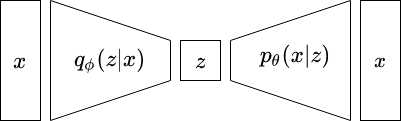
\includegraphics[width=0.6\textwidth]{vae}
  \caption{Estructura de un \textit{autoencoder} variacional}
  \label{fig:vae}
\end{figure}

\subsubsection{Función de coste}

Optimizando la función de coste se quiere conseguir que la aproximación $q_{\boldsymbol{\phi}}(\textbf{z}|\textbf{x})$ sea lo más cercana posible a la verdadera distribución a posteriori $p_{\boldsymbol{\theta}}(\textbf{z}|\textbf{x})$. Para ello debe introducirse una medida de la similitud entre dos funciones de distribución, la divergencia de Kullback-Leibler~\cite{kullback1997information}.

\begin{definicion}Dadas dos distribuciones de probabilidad P y Q sobre el mismo espacio de probabilidad, se define la \textit{divergencia de Kullback-Leibler} como $$D_{KL}(Q \parallel P) = E_Q \left[ \log \frac{Q(x)}{P(x)} \right].$$
\end{definicion}

\begin{proposicion}Dadas dos distribuciones de probabilidad P y Q sobre el mismo espacio de probabilidad, se cumple que $$D_{KL}(Q \parallel P) \geq 0.$$
\end{proposicion}\label{DKL-norm}

Realizamos también el cálculo de la divergencia entre dos distribuciones normales, que será útil para calcular la expresión concreta de la función de coste.

\begin{proposicion} Dadas las distribuciones de probabilidad  $p(\textbf{x}) = N(\textbf{x};\boldsymbol{\mu}_1, \boldsymbol{\Sigma}_1) $ y $q(\textbf{x}) = N(\textbf{x};\boldsymbol{\mu}_2, \boldsymbol{\Sigma}_2)$, ambas de dimensión $k$,
se cumple que $D_{KL}(p(\textbf{x}) \parallel q(\textbf{x})) = \frac{1}{2} \left( \log \frac{|\boldsymbol{\Sigma}_1|}{|\boldsymbol{\Sigma}_2|} - k + tr(\boldsymbol{\Sigma}_2^{-1}\boldsymbol{\Sigma}_1) + (\boldsymbol{\mu}_2 - \boldsymbol{\mu}_1)^T \boldsymbol{\Sigma}_2^{-1} (\boldsymbol{\mu}_2 - \boldsymbol{\mu}_1) \right).$\end{proposicion}

\begin{proof}
Comenzamos tomando el logaritmo de las funciones de densidad: $$ \log p(\textbf{x}) = -\frac{k}{2}\log(2 \pi) - \frac{1}{2} \vert \boldsymbol{\Sigma}_1\vert - \frac{1}{2}(\textbf{x} - \boldsymbol{\mu}_1)^T\boldsymbol{\Sigma}_1^{-1}(\textbf{x} - \boldsymbol{\mu}_1),$$ $$ \log p(\textbf{x}) = -\frac{k}{2}\log(2 \pi) - \frac{1}{2} \vert \boldsymbol{\Sigma}_2\vert - \frac{1}{2}(\textbf{x} - \boldsymbol{\mu}_2)^T\boldsymbol{\Sigma}_2^{-1}(\textbf{x} - \boldsymbol{\mu}_2).$$

Podemos entonces sustituir en la expresión de la divergencia de Kullback-Leibler:

$$D_{KL}(Q \parallel P) = E_p \left[ \log \frac{p(x)}{q(x)} \right] = E_p \left[ \log p(x) - \log q(x) \right] =$$

$$ E_p \left[- \frac{1}{2} \log \frac{\vert \boldsymbol{\Sigma}_2\vert}{\vert \boldsymbol{\Sigma}_1\vert} - \frac{1}{2}(\textbf{x} - \boldsymbol{\mu}_1)^T\boldsymbol{\Sigma}_1^{-1}(\textbf{x} - \boldsymbol{\mu}_1) + \frac{1}{2}(\textbf{x} + \boldsymbol{\mu}_2)^T\boldsymbol{\Sigma}_2^{-1}(\textbf{x} - \boldsymbol{\mu}_2) \right] = $$ $$E_p \left[- \frac{1}{2} \log \frac{\vert \boldsymbol{\Sigma}_2\vert}{\vert \boldsymbol{\Sigma}_1\vert}\right] - E_p\left[ \frac{1}{2}(\textbf{x} - \boldsymbol{\mu}_1)^T\boldsymbol{\Sigma}_1^{-1}(\textbf{x} - \boldsymbol{\mu}_1)\right]  + E_p\left[\frac{1}{2}(\textbf{x} + \boldsymbol{\mu}_2)^T\boldsymbol{\Sigma}_2^{-1}(\textbf{x} - \boldsymbol{\mu}_2) \right] .$$

Calculando por separado los sumandos, en el primero podemos quitar la esperanza de la expresión puesto que se trata de una constante. En el segundo

$$ E_p\left[ \frac{1}{2}(\textbf{x} - \boldsymbol{\mu}_1)^T\boldsymbol{\Sigma}_1^{-1}(\textbf{x} - \boldsymbol{\mu}_1)\right] = E_p\left[ tr \left( \frac{1}{2}(\textbf{x} - \boldsymbol{\mu}_1)^T\boldsymbol{\Sigma}_1^{-1}(\textbf{x} - \boldsymbol{\mu}_1) \right) \right] = $$
$$ E_p\left[ tr \left( \frac{1}{2}(\textbf{x} - \boldsymbol{\mu}_1)^T(\textbf{x} - \boldsymbol{\mu}_1)\boldsymbol{\Sigma}_1^{-1} \right) \right] = tr \left( E_p\left[  \frac{1}{2}(\textbf{x} - \boldsymbol{\mu}_1)^T(\textbf{x} - \boldsymbol{\mu}_1)\boldsymbol{\Sigma}_1^{-1} \right] \right) =$$
$$ tr \left( E_p\left[ (\textbf{x} - \boldsymbol{\mu}_1)^T(\textbf{x} - \boldsymbol{\mu}_1) \right]\frac{1}{2} \boldsymbol{\Sigma}_1^{-1} \right) = tr \left( \boldsymbol{\Sigma}_1 \frac{1}{2} \boldsymbol{\Sigma}_1^{-1} \right) = tr\left(\frac{1}{2} I_k \right) = \frac{k}{2}.$$

En el tercer sumando

$$E_p\left[\frac{1}{2}(\textbf{x} + \boldsymbol{\mu}_2)^T\boldsymbol{\Sigma}_2^{-1}(\textbf{x} - \boldsymbol{\mu}_2) \right] =$$ $$E_p\left[\frac{1}{2}((\textbf{x} - \boldsymbol{\mu}_1) + (\boldsymbol{\mu}_1 - \boldsymbol{\mu}_2))^T\boldsymbol{\Sigma}_2^{-1}((\textbf{x} - \boldsymbol{\mu}_1) + (\boldsymbol{\mu}_1 - \boldsymbol{\mu}_2)) \right] = $$ $$ E_p \left[\frac{1}{2} (\textbf{x} - \boldsymbol{\mu}_1)^T\boldsymbol{\Sigma}_2^{-1}(\textbf{x} - \boldsymbol{\mu}_1) + (\textbf{x} - \boldsymbol{\mu}_1)^T\boldsymbol{\Sigma}_2^{-1}(\boldsymbol{\mu}_1 - \boldsymbol{\mu}_2) + \frac{1}{2} (\boldsymbol{\mu}_1 - \boldsymbol{\mu}_2)^T\boldsymbol{\Sigma}_2^{-1}(\boldsymbol{\mu}_1 - \boldsymbol{\mu}_2) \right] = $$ $$ \frac{1}{2} tr(\boldsymbol{\Sigma}_2^{-1}{\boldsymbol{\Sigma}_1}) + \frac{1}{2}(\boldsymbol{\mu}_1 - \boldsymbol{\mu}_2)^T\boldsymbol{\Sigma}_2^{-1}(\boldsymbol{\mu}_1 - \boldsymbol{\mu}_2) + 0. $$

Sustituyendo cada uno de los sumandos se obtiene el resultado buscado.

\end{proof}

Por lo tanto queremos minimizar la expresión $$D_{KL}(q_{\boldsymbol{\phi}}(\textbf{z}|\textbf{x}) \parallel p_{\boldsymbol{\theta}}(\textbf{z}|\textbf{x})) = E_{z \sim q_{\boldsymbol{\phi}} (\textbf{z}|\textbf{x})} \left[ \log \frac{q_{\boldsymbol{\phi}}(\textbf{z}|\textbf{x})}{p_{\boldsymbol{\theta}}(\textbf{z}|\textbf{x})} \right]=$$ $$ E_{z \sim q_{\boldsymbol{\phi}} (\textbf{z}|\textbf{x})} \left[ \log q_{\boldsymbol{\phi}}(\textbf{z}|\textbf{x}) - \log p_{\boldsymbol{\theta}}(\textbf{z}|\textbf{x}) \right].$$

Sustituyendo $p_{\boldsymbol{\theta}}(\textbf{z}|\textbf{x})$ según la regla de Bayes obtenemos $$ D_{KL}(q_{\boldsymbol{\phi}}(\textbf{z}|\textbf{x}) \parallel p_{\boldsymbol{\theta}}(\textbf{z}|\textbf{x})) = E_{z \sim q_{\boldsymbol{\phi}} (\textbf{z}|\textbf{x})} \left[ \log q_{\boldsymbol{\phi}}(\textbf{z}|\textbf{x}) - \log  \frac{p_{\boldsymbol{\theta}}(\textbf{x}|\textbf{z})p_{\boldsymbol{\theta}}(\textbf{z})}{p_{\boldsymbol{\theta}}(\textbf{x})}\right]=$$ $$ E_{z \sim q_{\boldsymbol{\phi}} (\textbf{z}|\textbf{x})} \left[ \log q_{\boldsymbol{\phi}}(\textbf{z}|\textbf{x}) - \log  p_{\boldsymbol{\theta}}(\textbf{x}|\textbf{z}) - \log p_{\boldsymbol{\theta}}(\textbf{z}) + \log p_{\boldsymbol{\theta}}(\textbf{x})\right].$$

Como $\log p_{\boldsymbol{\theta}}(\textbf{x})$ no depende de $\textbf{z}$ puede extraerse de la esperanza: $$ D_{KL}(q_{\boldsymbol{\phi}}(\textbf{z}|\textbf{x}) \parallel p_{\boldsymbol{\theta}}(\textbf{z}|\textbf{x})) - \log p_{\boldsymbol{\theta}}(\textbf{x}) =$$ $$ E_{z \sim q_{\boldsymbol{\phi}} (\textbf{z}|\textbf{x})} \left[ \log q_{\boldsymbol{\phi}}(\textbf{z}|\textbf{x}) - \log  p_{\boldsymbol{\theta}}(\textbf{x}|\textbf{z}) - \log p_{\boldsymbol{\theta}}(\textbf{z})\right].$$

Utilizando la linealidad de la esperanza:

$$ \log p_{\boldsymbol{\theta}}(\textbf{x}) - D_{KL}(q_{\boldsymbol{\phi}}(\textbf{z}|\textbf{x}) \parallel p_{\boldsymbol{\theta}}(\textbf{z}|\textbf{x})) =$$ $$ E_{z \sim q_{\boldsymbol{\phi}} (\textbf{z}|\textbf{x})} \left[ \log p_{\boldsymbol{\theta}}(\textbf{x}|\textbf{z}) \right] - E_{z \sim q_{\boldsymbol{\phi}} (\textbf{z}|\textbf{x})} \left[ \log  q_{\boldsymbol{\phi}}(\textbf{z}|\textbf{x}) - \log p_{\boldsymbol{\theta}}(\textbf{z})\right]=$$ $$ E_{z \sim q_{\boldsymbol{\phi}} (\textbf{z}|\textbf{x})} \left[ \log p_{\boldsymbol{\theta}}(\textbf{x}|\textbf{z}) \right] - D_{KL}(q_{\boldsymbol{\phi}}(\textbf{z}|\textbf{x}) \parallel p_{\boldsymbol{\theta}}(\textbf{z})).$$

La expresión anterior recibe el nombre de cota inferior de la evidencia (\textit{evidence lower bound}, ELBO), ya que a $\log p_{\boldsymbol{\theta}}(\textbf{x})$ se le llama evidencia y la divergencia de Kullback-Leibler siempre positiva. Por lo tanto la ELBO es siempre una cota inferior de la evidencia. Maximizando la expresión conseguimos, por un lado, maximizar $p_{\boldsymbol{\theta}}(\textbf{x})$, lo que se traduce en una mejor generación de ejemplos, y por otro minimizar la divergencia entre la aproximación $q_{\boldsymbol{\phi}}(\textbf{z}|\textbf{x})$ y la verdadera distribución a priori $p_{\boldsymbol{\theta}}(\textbf{z}|\textbf{x}))$~\cite{kingma2019introduction}.  Así, la función de coste a minimizar es $$L(\boldsymbol{\theta}, \boldsymbol{\phi}; \textbf{x}) = - E_{z \sim q_{\boldsymbol{\phi}} (\textbf{z}|\textbf{x})} \left[ \log p_{\boldsymbol{\theta}}(\textbf{x}|\textbf{z}) \right] + D_{KL}(q_{\boldsymbol{\phi}}(\textbf{z}|\textbf{x}) \parallel p_{\boldsymbol{\theta}}(\textbf{z})). $$

Podemos obtener la expresión concreta de la función de coste sustituyendo los valores de las distribuciones conocidas en la divergencia de Kullback-Leibler. Previamente se fijó que $p_{\boldsymbol{\theta}}(\textbf{z}) = \mathcal{N}(\textbf{z};\mathbf{0},\textbf{I})$ y $ q_{\boldsymbol{\phi}}(\textbf{z}|\textbf{x}) = \mathcal{N}(\textbf{z};\boldsymbol{\mu},\boldsymbol{\sigma}^{2}\textbf{I})$. Aplicando la \autoref{DKL-norm} $$ D_{KL}(q_{\boldsymbol{\phi}}(\textbf{z}|\textbf{x}) \parallel p_{\boldsymbol{\theta}}(\textbf{x})) = D_{KL}( \mathcal{N}(\boldsymbol{\mu},\boldsymbol{\sigma}^{2}\textbf{I}) \parallel \mathcal{N}(\mathbf{0},\textbf{I})) =$$ $$\frac{1}{2} \left( -\log|\boldsymbol{\sigma}^{2}\textbf{I}| -k + tr(\boldsymbol{\sigma}^{2}\textbf{I}) + \boldsymbol{\mu}^T\boldsymbol{\mu} \right)$$

donde $k$ es la dimensión de las distribuciones. Podemos simplificar esta expresión como $$D_{KL}(q_{\boldsymbol{\phi}}(\textbf{z}|\textbf{x}) \parallel p_{\boldsymbol{\theta}}(\textbf{x})) =  \frac{1}{2} \left( -\log|\boldsymbol{\sigma}^{2}\textbf{I}| -k + tr(\boldsymbol{\sigma}^{2}\textbf{I}) + \boldsymbol{\mu}^T\boldsymbol{\mu} \right) = $$

$$\frac{1}{2} \left( -\log (\prod_{j=1}^{k}\sigma_j^{2}) -\sum_{j=1}^k 1 + \sum_{j=1}^k \sigma_j^2 + \sum_{j=1}^k \mu_j^2 \right) =$$ $$\frac{1}{2} \left( -\sum_{j=1}^k\log (\sigma_j^{2}) -\sum_{j=1}^k 1 + \sum_{j=1}^k \sigma_j^2 + \sum_{j=1}^k \mu_j^2 \right) = $$ $$ \frac{1}{2}\sum_{j=1}^k \left( -log(\sigma_j^2) -1 + \sigma_j^2 + \mu_j^2 \right).$$ Sustituyendo en la expresión original, la función de coste definitiva es

$$L(\boldsymbol{\theta}, \boldsymbol{\phi}; \textbf{x}) = - E_{z \sim q_{\boldsymbol{\phi}} (\textbf{z}|\textbf{x})} \left[ \log p_{\boldsymbol{\theta}}(\textbf{x}|\textbf{z}) \right] +  \frac{1}{2}\sum_{j=1}^k \left( -log(\sigma_j^2) -1 + \sigma_j^2 + \mu_j^2 \right). $$

\subsubsection{Optimización}

Existe un problema para aplicar los algoritmos de optimización vistos en la \autoref{optimizacion}. La función de coste incluye un proceso de muestreo de la distribución $q_{\boldsymbol{\phi}} (\textbf{z}|\textbf{x})$, por lo que no puede calcularse su gradiente. Para poder calcularlo se utiliza, en lugar de $E_{z \sim q_{\boldsymbol{\phi}} (\textbf{z}|\textbf{x})} \left[ \log p_{\boldsymbol{\theta}}(\textbf{x}|\textbf{z}) \right]$, un estimador mediante el truco de reparametrización~\cite{kingma2013auto}.

Este consiste en expresar $\textbf{z}^{(l)} \sim q_{\boldsymbol{\phi}} (\textbf{z}|\textbf{x})$ mediante una transformación diferenciable de una variable aleatoria $\epsilon \sim \mathcal{N}(\boldsymbol{0}, \textbf{I})$ que actúa como ruido, $$ \textbf{z}^{(l)} = g_{\boldsymbol{\phi}}(\textbf{x}, \boldsymbol{\epsilon}^{(l)}) = \boldsymbol{\mu} + \boldsymbol{\sigma} \odot \boldsymbol{\epsilon}^{(l)},$$ donde $\boldsymbol{\mu}$ y $\boldsymbol{\sigma}$ son tales que $q_{\boldsymbol{\phi}}(\textbf{z}|\textbf{x}) = \mathcal{N}(\textbf{z};\boldsymbol{\mu},\boldsymbol{\sigma}^{2}\textbf{I})$. Así, el estimador de la función de coste para el punto $\textbf{x}^{(i)}$ será $$\tilde{L}(\boldsymbol{\theta}, \boldsymbol{\phi}; \textbf{x}) = -\frac{1}{\mathcal{L}}\sum_{l=1}^{\mathcal{L}}\log p_{\boldsymbol{\theta}}(\textbf{x}^{(i)}|\textbf{z}^{(i,l)}) +  \frac{1}{2}\sum_{j=1}^k \left( -log(\sigma_j^2) -1 + \sigma_j^2 + \mu_j^2 \right).$$

Dado un conjunto $\textbf{X}$ con $N$ datos, puede construirise un estimador del conjunto entero, basado en minilotes: $$ \tilde{L}(\boldsymbol{\theta}, \boldsymbol{\phi}; \textbf{X}) = \tilde{L}^M(\boldsymbol{\theta}, \boldsymbol{\phi}; \textbf{X}^M) = \frac{N}{M} \sum_{i=1}^{M} \tilde{L}^M(\boldsymbol{\theta}, \boldsymbol{\phi}; \textbf{x}^{(i)})$$ donde el minilote $\textbf{X}^M = \{\textbf{x}^{(i)}\}^M_{i=1}$ es un subconjunto de M elementos de \textbf{X} elegidos aleatoriamente. La aplicación en el entrenamiento se detalla en el algoritmo \autoref{minibatch-AEVB}.

\begin{algorithm}
\label{minibatch-AEVB}
 \caption{Versión con minilotes del algoritmo .}
     \SetAlgoLined
     $\boldsymbol{\theta}$, $\boldsymbol{\phi}$ $\leftarrow$ Inicializa parámetros\;
     \While{los parámetros $\boldsymbol{\theta}$, $\boldsymbol{\phi}$ no convergen}{
     $\textbf{X}^M$ $\leftarrow$ Minilote aleatorio de M datos\;
     $\boldsymbol{\epsilon}$ $\leftarrow$ Muestras aleatorias de la distribución de ruido\;
     $\boldsymbol{g}$ $\leftarrow$ $\nabla_{\boldsymbol{\theta}, \boldsymbol{\phi}} \tilde{L}^M(\boldsymbol{\theta}, \boldsymbol{\phi}; \textbf{x}^{(i)})$\;
     $\boldsymbol{\theta}$, $\boldsymbol{\phi}$ $\leftarrow$ Actualiza los parámetros mediante un algoritmo basado en gradiente
     }
     $\textbf{y} \leftarrow \textbf{h}_{\ell}$\;
\end{algorithm}



\endinput
%------------------------------------------------------------------------------------
% FIN DEL CAPÍTULO.
%------------------------------------------------------------------------------------
